

\cleardoublepage

\addcontentsline{toc}{chapter}{\numberline{}Preeemiiiiier chapiter}
\addtocontents{lof}{\textbf{Chapter A1}}

\setcounter{chapter}{1}



\begin{center}
	\Huge\textbf{premier chapter}
\end{center}

\section{Introduction}
L’une des récentes avancées dans la micro électronique et des technologies sans-fil qui confortent la présence de l’informatique et de l’électronique au cœur du monde réel ont permis de développer des capteurs de petite taille. Ces  micro-capteurs sont dotés d’une capacités de traitement permettant de collecter et de transmettre des données environnementales d'une manière autonome.Les réseaux de capteurs sans fil ou WSNs(Wireless Sensor Networks) sont constitués d’un ensemble de capteurs sans fil s’auto organisant pour acquérir des données de leur environnement immédiat, de les traiter et de les communiquer.
Dans ce premier chapitre, nous présenterons un ensemble de généralités sur les réseaux de capteurs, notamment sur leur architecture et leurs domaines d’applications.\\

\section{Un réseau de capteur sans-fil}
un réseau de capteur sans fil est un type spécial de réseau ad-hoc où la plupart de ces nœuds sont des micro-capteurs dispersés dans une zone géographique appelée zone de captage. La position de ces nœuds n’est pas obligatoirement déterminée, ils utilisent une communication sans fil pour acheminer les données captées avec un routage multi sauts vers un nœud collecteur appelé nœud puits(Sink). Ces capteurs comme ils ont été décrit au paravent  sont des diapositifs de taille extrêmement réduite avec des sources limitées, autonome, capable de traiter et transmettre les informations.

\begin{figure}[h]
	\centering
	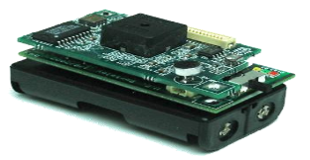
\includegraphics[width=7cm,height=3.7cm]{Chap1/1.png}
	\caption{Capteur sans fils}
	\label{fig:CSF}
\end{figure}

Les réseaux de capteurs utilisent un très grand nombre de ces capteurs, pour former un réseau sans infrastructure établie. Chaque capteur relayant l'information sur sa propre zone de couverture, le réseau se trouve entièrement couvert.

\begin{figure}[h]
	\centering
	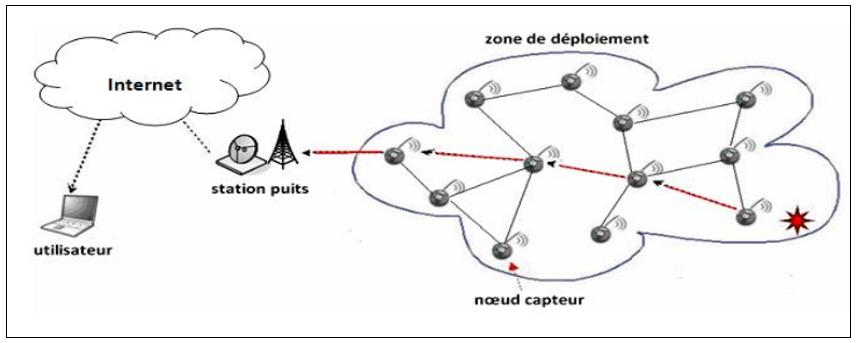
\includegraphics[width=14cm,height=6cm]{Chap1/2.png}
	\caption{Architecture d’un réseau de capteurs sans fil}
	\label{fig:ARCSF}
\end{figure}

\section{Architecture d’un capteur sans-fil}
Un capteur est composé de quatre composants de base: Unité d’acquisition peut être nommé aussi unité de capture, unité de traitement, unité de communication(unité d'émission/réception), et une unité d'énergie. 
Il se peut aussi qu'il existe d'autres composants additionnels dépendant de l'application, par exemples: un générateur d'énergie, un système de localisation, et un mobilisateur.\cite{mekidicheetude}

\begin{figure}[h]
	\centering
	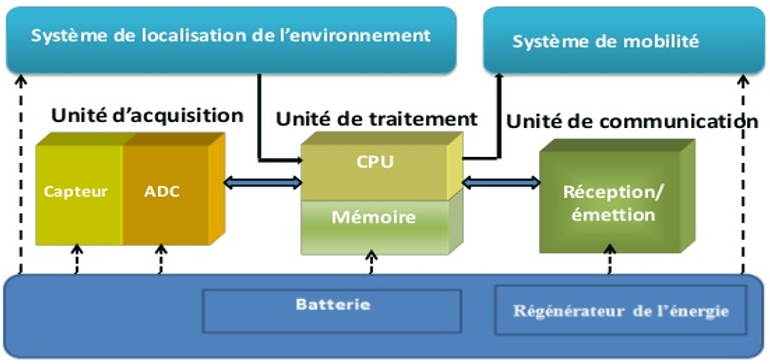
\includegraphics[width=14cm,height=6cm]{Chap1/3.png}
	\caption{Architecture d’un nœud capteur}
	\label{fig:ANC}
\end{figure}

\begin{itemize}
  \item \textbf{Unité d’acquisition: }se compose généralement de deux sous unités: un capteur et un convertisseur(ADC) (analogique,numérique).
Les signaux analogiques mesurés par le capteur sont convertis en signaux numériques (digitaux) et sont transmis à l’unité de traitement \cite{mekidicheetude}.
 
  \item \textbf{Unité de traitement: }L’unité de traitement, comprend un processeur associé généralement à une petite unité de stockage et fonctionne à l’aide d’un système d’exploitation spécialement conçu pour les micro-capteurs (TinyOS \cite{hill2000system}, par exemple). Cette unité est chargée d’exécuter les protocoles de communication qui permettent la collaboration entre les capteurs du réseau; Elle peut aussi analyser les données captées pour alléger la tâche des stations puits. De plus, l’unité de traitement nécessite un stockage pour minimiser la taille des messages transmis et cela en appliquant un traitement local et une agrégation de données \cite{feng2002system}.
	\item \textbf{Unité de communication: }cette unité est responsable de l’émission et de la réception au moyen de support sans fil. Il existe trois schéma de communication pour les réseaux de capteurs : La communication optique (laser), L’infrarouge et la communication par fréquence radio. D’après les recherches scientifique la communication optique consomme moins d’énergie que la communication qui utilise la fréquence radio, son inconvénient est l’utilisation  d’une ligne optique qui est sensible à la perturbation physique. L’infrarouge a une capacité de diffusion très limitée et il n’a pas besoin de l’antenne contrairement au fréquence radio qui utilise des antennes mais très simple à l’utiliser.
	\item \textbf{Unité de contrôle d’énergie(batterie): }c’est l’unité la plus importante. Son rôle est de distribuer de manière équitable l'énergie disponible entre les différentes unités et de réduire les dépenses en mettant en veille les composants inactifs
\begin{figure}[H]
	\centering
	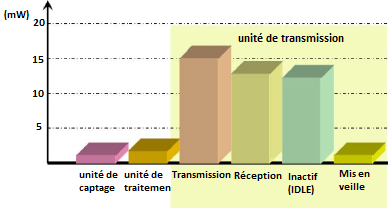
\includegraphics[width=14cm,height=6cm]{Chap1/4.png}
	\caption{Consommation d’énergie dans un nœud capteur. \cite{raghunathan2005design,karl2007protocols}}
	\label{fig:CENC}
\end{figure}
\end{itemize}

\section{Architecture d’un réseau de capteurs sans-fil}
La plupart des architectures communes à un WSN suivent le modèle OSI. En principe, dans le réseau de capteurs, nous avons besoin de cinq couches: couche application, couche de transport, couche réseau, couche liaison de données et couche physique. Les cinq couches sont complétées par les plans des trois couches, comme illustré à la Figure. 1.5 .
\begin{figure}[h]
	\centering
	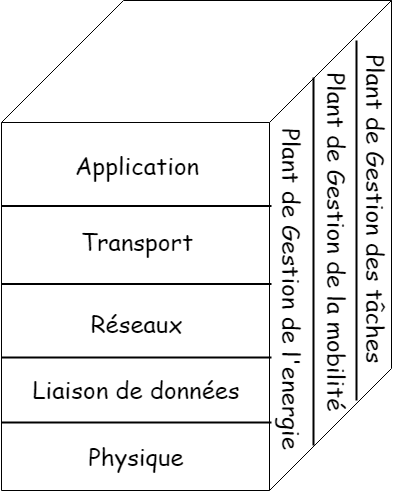
\includegraphics[width=11cm,height=7cm]{Chap1/5.png}
	\caption{L’architecture d’un WSN}
	\label{fig:AWSN}
\end{figure}


\subsection{Les couches WSN OSI}
\begin{itemize}
	\item \textbf{La couche physique: }La fonction de cette couche est d'assurer la fiabilité et d’éviter la congestion, où beaucoup de protocoles conçus pour assurer cette fonction sont soit appliquée en amont ou en aval. Ces protocoles utilisent des mécanismes différents pour la détection des pertes et la récupération des pertes [7, 8]. Cette couche est particulièrement nécessaire lorsqu'un système est organisé pour accéder à d'autres réseaux.
	
	\item \textbf{La couche liaison de données: }Cette couche a pour rôle le multiplexage des flux de données, le partage de l’accès au medium et le contrôle d’erreur. Elle assure une connexion point a point ou point a multipoint fiable dans une communication réseau. \cite{bachir2010mac,meghan2009comparative} Elle est composée de deux couches: la couche LLC (Contrôle des Liens Logiques) et la couche MAC (Contrôle d’accès au medium). Les protocoles de la sous couche MAC sont appelés à effectuer d’importantes opérations citant :
	\begin{itemize}
		\item Etablir des liens de communication entre les nœuds capteurs voisins.
		\item Fournir une fiabilité entre ces nœuds voisins.
		\item Partager équitablement les canaux de communication entre les nœuds du 		réseau.
	\end{itemize}

	\item \textbf{La couche réseau: }La fonction principale de cette couche est le routage. Cette couche présente de nombreux défis en fonction de l’application, mais apparemment, les principaux problèmes sont les suivants: économie d’énergie, mémoire et tampons limités, le capteur n’a pas d’ID global et doit être auto-organisé. C’est différent des réseaux informatiques avec adresse IP et dispositif central de commande \cite{akyildiz2002wireless,akyildiz2007survey}.
	
	\item \textbf{La couche transport:  }Cette couche est responsable du maintien des flux de données dans les applications utilisées et de la sauvegarde des données dans le cache des capteurs. Elle est particulièrement nécessaire pour accéder au réseau de capteurs par le biais d’un réseau externe comme l’internent \cite{nieberg2003collaborative}. A l’instar des autres couches, de nouvelles approches doivent être mises en place pour faire face aux contraintes inhérentes à ce type de réseau.
	
	\item \textbf{La couche application: }Cette couche est responsable de la gestion des trafic. Elle permet d’envoyer des requête pour récupérer certaines informations ainsi de fournir des logiciels pour toutes les applications qui traduisent les données sous une forme compréhensible. 

\end{itemize}


\subsection{Les plans de gestion de la pile protocolaire:}
En plus des cinq couches, la pile protocolaire dans un réseau de capteurs comporte trois plans de gestion de l’énergie ou couches transversaux qui sont: plan de gestion de l’énergie, plan de gestion de la mobilité et plan de gestion des tâches. 
Ces couches servent à gérer le réseau et à faire en sorte que les capteurs fonctionnent ensemble afin d'accroître l'efficacité globale du réseau\cite{akyildiz2002wireless}.

\begin{itemize}
	\item \textbf{Le plan de gestion d’énergie: }ce plan gère la consommation d’énergie par les capteurs.
	\item \textbf{Le plan de gestion de la mobilité: }ce niveau enregistre le mouvement des nœuds capteurs et détecte leurs position, permet de maintenir l’itinéraire d’un capteur vers un utilisateur et garde la trace de l’emplacement de ses voisins.
	\item \textbf{Le plan de gestion des taches : }s’occupe de la répartition des taches pour une région donnée.
\end{itemize}


\section{Domaines d'application des réseaux de capteurs}
Les WSNs trouvent leurs intérêts dans des applications diverses et innovatrices. Le champs d’application des réseaux de capteurs est devenu très large grâce à la diminution des coûts de fabrication des micro-capteurs,leurs taille réduite, l’absence des cables entre les nœuds,  l'élargissement de la gamme des types de capteurs disponibles (thermique, optique, vibrations, ... ) et l'évolution des support de communication sans fil.

\subsection{Domaine militaire}
Comme dans le cas de plusieurs technologies, le domaine militaire a été un moteur d'origine 	pour le développement des réseaux de capteurs. Le déploiement rapide, le coût réduit, l'auto-	organisation et la tolérance aux pannes des réseaux de capteurs sont des caractéristiques qui 	rendent ce type de réseaux un outil appréciable dans un tel domaine. \cite{mekidicheetude}
	Un réseau de capteurs déployé sur un secteur stratégique ou complexe d'accès, permet par 	exemple la surveillance du champ de bataille, détection des attaques Nucléaires, Biologiques 	et chimiques, estimation des dommages ainsi que la reconnaissance des forces opposées et 	du terrain. 
\begin{figure}[h]
	\centering
	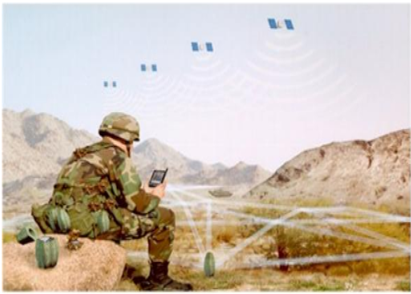
\includegraphics[width=9cm,height=4cm]{Chap1/6.png}
	\caption{surveillance militaire}
	\label{fig:SM}
\end{figure}

\subsection{Domaine médicale}
Les réseaux de capteurs sont largement répandus dans le domaine médical, incluant des 	applications comme : collecter des informations de meilleure qualité facilitant ainsi le diagnostic de quelques maladies et aussi l’intervention rapide si les mesures effectuées par 	les capteurs sont anormales, surveiller des fonctions vitales d'un organisme vivant pourrait à 	l'avenir être facilitée par des micro-capteurs avalés ou implantés sous la peau ,fournir une 	interface d'aide pour les handicapés, collecter des informations physiologiques humaines de 	meilleure qualité, surveiller en permanence les malades et les médecins à l'intérieur de 	l'hôpital.
\begin{figure}[h]
	\centering
	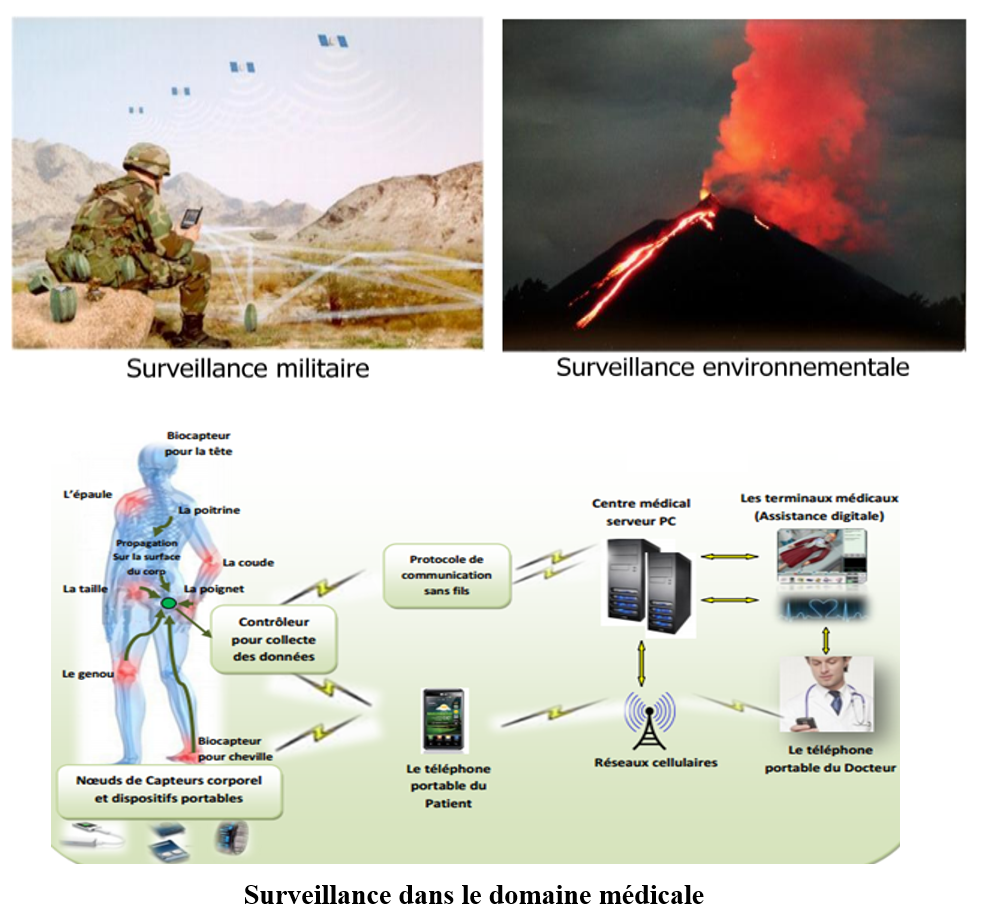
\includegraphics[width=12cm,height=4cm]{Chap1/7.png}
	\caption{surveillance médicale}
	\label{fig:SM}
\end{figure}

\subsection{Domaine environnementale}
Dans ce domaine, les capteurs peuvent êtres exploités pour suivre du déplacement des 	oiseaux, de petits animaux et d’insecte,détecter les catastrophes naturelles (feux de forêts, 	tremblements de terre, etc.), connaître la qualité de l’air et détecter la pollution, détecter des 	fuites des produits toxiques (gaz, produits chimiques, pétrole, etc.) dans des sites industriels 	tels que les centrales nucléaires et les pétrolières. Les réseaux capteurs peuvent même être 	utilisé dans la recherche météorologique et géophysique.
\begin{figure}[h]
	\centering
	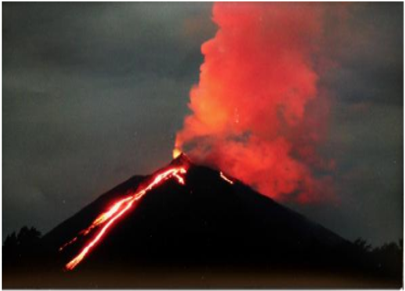
\includegraphics[width=12cm,height=6cm]{Chap1/8.png}
	\caption{surveillance environnementale}
	\label{fig:SM}
\end{figure}

\subsection{Domaine commercial}
Les réseaux de capteurs ont prouvé leurs utilité dans le domaine commercial. Dans ce 	domaine on peut énumérer plusieurs applications citant: contrôler le stockage des produit 	ainsi que leurs livraison (concernant la chaîne du froid), suivre le procédé de production 	d’un produit (tous les étapes), contrôler et automatiser le processus d’usinage, ect. Pour 	amélioré la qualité de service d’une entreprise en terme de livraison on peut même offrir à 	un client la possibilité de suivre le  paquet qu’il attend en temps réel et connaître la position 	de ce dernier.


\section{Le problème majeur d’un réseau de capteurs sans fil et le challenge:}
L'un des défis auxquels est confronté un réseau de capteurs sans fil (WSN) est la dissipation d'énergie des nœuds ayant une incidence sur la durée de vie de la batterie du nœud. Cela est dû au fait que les nœuds plus proches de nœud puits supportent des charges de trafic plus lourdes que tout autre nœud. Par conséquent, les nœuds autour du nœud puits épuiseraient leur énergie plus rapidement ce qui cause par la suite ce qu’on appel un trou d’énergie. Après cela, les données ne peuvent plus être transmises, même s'il reste encore de l'énergie dans les nœuds de la région externe, ce qui affecte la durée de vie du réseau. Comme les réseaux de capteur sont utilisés pour des tâches critique, pensé à l’optimisation ou à la conservation de  l’énergie pour chaque nœud capteur est une conséquence très probable.
Dans la littérature, le concept d’ensemble dominant connecté \cite{guha1998approximation,park2007dominating,thai2008construction,wan2002distributed} a été étudié pour la construction d’une ossature de routage avec une consommation d’énergie minimale dans les WSNs. Ces papiers considèrent le poids sur chaque nœud au lieu du poids sur chaque bord. Ceci a conduit à l'introduction du problème de l’arbre dominant DTP \cite{shin2010approximation,zhang2008new} avec l'objectif de prolonger la durée de vie d’un capteur. \cite{sundar2014steady}
Le DTP semble résoudre le problème de la consommation de l’énergie mais ce dernier et gourmand en terme de temps d’exécution. Pour ce problème, les chercheurs ont pensé à l’approximation de ce problème en un problème polynomial et ils ont développé des algorithmes  d’optimisation qui visent à construire un arbre dominant dans un temps minimal, nommé les méthodes approchées, tous ces détails seront exploité dans les prochains chapitres.

\section{Conclusion:}
Un réseau de capteurs est constitué de plusieurs nœuds capteurs capables  de collecter et de traiter des informations sur l'environnement dans lequel ils sont déployés et de les transmettre vers un site donné (station). Ils se caractérisent par une grande flexibilité et tolérance aux fautes. Grâce à ces caractéristiques le champ d'application des réseaux de capteurs s'est étendu pour contenir la plupart des domaines tels que l’industrie, la recherche, l’environnement, la médecine ainsi que le domaine militaire. Cependant, L’apparition de ce type de réseaux a engendré plusieurs défis notamment pour la résolution du problème de trou d’énergie. Plusieurs solution ont été proposer pour cela, mentionnant le calcule de l’arbre dominant, un problème Np-Hard, nécessite pour sa résolution les méta-heuristiques qui sont considérées comme les meilleurs approches d’optimisation; des détails explicatifs font l’objet de notre prochain chapitre.


